\chapter{Vector Calculus}

\section{Function ($f(x)$)}

\begin{enumerate}
    \item A function $f$ is a quantity that relates two quantities to each other. 
    \hfill \cite{mfml/book/mml/Deisenroth-Faisal-Ong}

    \item These quantities are typically inputs $\bm{x} \in \mathbb{R}^D$ and targets (function values) $f (\bm{x})$, which we assume are real-valued if not stated otherwise. 
    \hfill \cite{mfml/book/mml/Deisenroth-Faisal-Ong}
    
    \item $\mathbb{R}^D$ is the domain of $f$ , and the function values $f (\bm{x})$ are the image/codomain of $f$ .
    \hfill \cite{mfml/book/mml/Deisenroth-Faisal-Ong}

    \item We often write 
    \hfill \cite{mfml/book/mml/Deisenroth-Faisal-Ong}
    \begin{enumerate}
        \item $f: \mathbb{R}^D \to \mathbb{R}$ 
        (specifies that $f$ is a mapping from $\mathbb{R}^D$ to $\mathbb{R}$ )
        \hfill \cite{mfml/book/mml/Deisenroth-Faisal-Ong}
        
        \item $\bm{x} \mapsto f(\bm{x})$ 
        (specifies the explicit assignment of an input $\bm{x}$ to a function value $f(\bm{x})$)
        \hfill \cite{mfml/book/mml/Deisenroth-Faisal-Ong}
    \end{enumerate}
    to specify a function.
    \hfill \cite{mfml/book/mml/Deisenroth-Faisal-Ong}

    \item A function $f$ assigns every input x exactly one function value $f (\bm{x})$.
    \hfill \cite{mfml/book/mml/Deisenroth-Faisal-Ong}
\end{enumerate}

\vspace{0.5cm}
\textbf{ALSO SEE/ RELATED}:
\begin{enumerate}
    \item \fullref{vector space/Linear Mappings}
\end{enumerate}



\subsection{Differentiation of Uni-variate Functions}

\begin{enumerate}
    \item 
    \begin{definition}[Univariate function ($f : \mathbb{R} \to \mathbb{R}$)]
        Univariate function: $y = f(x),\ x, y \in \mathbb{R}$
        \hfill \cite{mfml/book/mml/Deisenroth-Faisal-Ong}
    \end{definition}

    \item 
    \begin{definition}[Difference Quotient]
        The difference quotient
        $
            \dfrac{\delta y}{\delta x} 
            := \dfrac{f(x + \delta x) - f(x)}{\delta x}
        $
        computes the slope of the secant line through two points on the graph of $f$ .
        \hfill \cite{mfml/book/mml/Deisenroth-Faisal-Ong}
    \end{definition}

    \item The derivative of $f$ points in the direction of steepest ascent of $f$. 
    \hfill \cite{mfml/book/mml/Deisenroth-Faisal-Ong}

    \item 
    \begin{definition}[Taylor Polynomial ( $T_n(x)$ )]
        The Taylor polynomial of degree $n$ of $f : \mathbb{R} \to \mathbb{R}$ at $x_0$ is defined as
        $
            T_n(x)
            := \dsum_{k=0}^n \dfrac{f^{(k)}(x_0)}{k!} (x - x_0)^k
        $
        \hfill \cite{mfml/book/mml/Deisenroth-Faisal-Ong}
        \\
        where $f ^{(k)}(x_0)$ is the $k$-th derivative of $f$ at $x_0$ (which we assume exists) and $\dfrac{f ^{(k)}(x_0)}{ k!}$ are the coefficients of the polynomial.
        \hfill \cite{mfml/book/mml/Deisenroth-Faisal-Ong}
        \\
        We define $t^0 := 1$ for all $t \in \mathbb{R}$.
        \hfill \cite{mfml/book/mml/Deisenroth-Faisal-Ong}
    \end{definition}
    \begin{enumerate}
        \item In general, a Taylor polynomial of degree $n$ is an \textbf{approximation} of a function, which does not need to be a polynomial. 
        The Taylor polynomial is similar to $f$ in a neighborhood around $x_0$. 
        Higher-order Taylor polynomials approximate the function $f$ better and more globally.
        \hfill \cite{mfml/book/mml/Deisenroth-Faisal-Ong}
        
        \item A Taylor polynomial of degree $n$ is an \textbf{exact} representation of a polynomial $f$ of degree $k \leq n$ since all derivatives $f (i)$, $i > k$ vanish. 
        \hfill \cite{mfml/book/mml/Deisenroth-Faisal-Ong}
    \end{enumerate}


    \item 
    \begin{definition}[Power Series]
        $
            f(x) = \dsum_{k=0}^{\infty} a_k (x-c)^k
        $
        \\
        where $a_k$ are coefficients and $c$ is a constant
    \end{definition}


    \item 
    \begin{definition}[Taylor Series ($T_{\infty}(x)$)]
        For a smooth function $f \in C^{\infty}$, $f : \mathbb{R} \to \mathbb{R}$, the Taylor series of $f$ at $x_0$ is defined as
        $
            T_{\infty}(x)
            = \dsum_{k=0}^{\infty} \dfrac{f^{(k)}(x_0)}{k!} (x - x_0)^k
        $
        \hfill \cite{mfml/book/mml/Deisenroth-Faisal-Ong}
        \\
         $f \in C^{\infty}$ means that $f$ is continuously differentiable infinitely many times
         \hfill \cite{mfml/book/mml/Deisenroth-Faisal-Ong}
    \end{definition}
    \begin{enumerate}
        \item 
        \begin{definition}[Maclaurin series]        
            For $x_0 = 0$, we obtain the \textbf{Maclaurin series} as a special instance of the Taylor series. 
            \hfill \cite{mfml/book/mml/Deisenroth-Faisal-Ong}
        \end{definition}

        \item 
        \begin{definition}[Analytic]        
            If $f (x) = T_{\infty}(x)$, then $f$ is called \textbf{analytic}.
            \hfill \cite{mfml/book/mml/Deisenroth-Faisal-Ong}
        \end{definition}
    \end{enumerate}
\end{enumerate}




\subsection{Differentiation of multi-variate Functions}

\begin{enumerate}
    \item 
    \begin{definition}[multi-variate Functions ($f : \mathbb{R}^n \to \mathbb{R}$)]
        The general case where the function $f$ depends on one or more variables $\bm{x} \in \mathbb{R}^n$
        \hfill \cite{mfml/book/mml/Deisenroth-Faisal-Ong}
    \end{definition}

    \item 
    \begin{definition}[Partial Derivative ($\dfrac{\partial f}{\partial x_i}$)]
        For a function $f : \mathbb{R}^n \to \mathbb{R}$, $\bm{x} \mapsto f (\bm{x})$, $\bm{x} \in \mathbb{R}^n$ of $n$ variables $x_1, \cdots , x_n$ we define the partial derivatives as
        \hfill \cite{mfml/book/mml/Deisenroth-Faisal-Ong}
        \\
        .\hfill
        ${
            \displaystyle
            \begin{matrix}
                \dfrac{\partial f}{\partial x_1} 
                & 
                = 
                & 
                \lim_{h\to 0} \dfrac{f (x_1 + h, x_2, \cdots , x_n) - f (\bm{x})}{h}
                \\
                & \vdots &
                \\
                \dfrac{\partial f}{\partial x_n} 
                & 
                = 
                & 
                \lim_{h\to 0} \dfrac{f (x_1 , x_2, \cdots , x_n+ h) - f (\bm{x})}{h}
            \end{matrix}
        }$
        \hfill \cite{mfml/book/mml/Deisenroth-Faisal-Ong}
    \end{definition}
\end{enumerate}

\subsubsection{Gradient}

\begin{enumerate}
    \item The generalization of the derivative to functions of several variables is the \textbf{gradient}.
    \hfill \cite{mfml/book/mml/Deisenroth-Faisal-Ong}

    \item We find the gradient of the function $f$ with respect to $\bm{x}$ by varying one variable at a time and keeping the others constant. 
    \hfill \cite{mfml/book/mml/Deisenroth-Faisal-Ong}
    
    \item The gradient is then the \textbf{collection} of these partial derivatives.
    \hfill \cite{mfml/book/mml/Deisenroth-Faisal-Ong}

    \item 
    \begin{definition}[Gradient ($\nabla_x f \in \mathbb{R}^{1 \times n}$)]
        For a function $f : \mathbb{R}^n \to \mathbb{R}$, $\bm{x} \mapsto f (\bm{x})$, $\bm{x} \in \mathbb{R}^n$ of $n$ variables $x_1, \cdots , x_n$:
        \\
        .\hfill
        $
            \nabla_x f
            = \text{grad} f
            = \dfrac{df}{d\bm{x}}
            = \begin{bmatrix}
                \dfrac{\partial f(\bm{x})}{\partial x_1} &
                \dfrac{\partial f(\bm{x})}{\partial x_2} &
                \cdots
                \dfrac{\partial f(\bm{x})}{\partial x_n}
            \end{bmatrix}
            \in \mathbb{R}^{1 \times n}
        $
        \hfill \cite{mfml/book/mml/Deisenroth-Faisal-Ong}
        \\
        where $n$ is the number of variables and $1$ is the dimension of the image/range/codomain of $f$ .
        The row vector is called the gradient of $f$ or the Jacobian.
        \hfill \cite{mfml/book/mml/Deisenroth-Faisal-Ong}
    \end{definition}

    \item This definition of Jacobian is a special case of the general definition of the Jacobian for vector-valued functions as the collection of partial derivatives.
    \hfill \cite{mfml/book/mml/Deisenroth-Faisal-Ong}

    \item The reason why we define the gradient vector as a row vector:
    \hfill \cite{mfml/book/mml/Deisenroth-Faisal-Ong}
    \begin{enumerate}
        \item we can consistently generalize the gradient to vector-valued functions $f : \mathbb{R}^n \to \mathbb{R}^m$ (then the gradient becomes a matrix)
        \hfill \cite{mfml/book/mml/Deisenroth-Faisal-Ong}

        \item we can immediately apply the multi-variate chain rule without paying attention to the dimension of the gradient.
        \hfill \cite{mfml/book/mml/Deisenroth-Faisal-Ong}
    \end{enumerate}
\end{enumerate}






\section{Gradients of Vector-Valued Functions ($\nabla_x f$)}

\begin{enumerate}
    \item 
    \begin{definition}[vector-valued functions/ vector fields ($\bm{f} : \mathbb{R}^n \to \mathbb{R}^m$)]
        vector-valued functions (vector fields) are defined as $\bm{f} : \mathbb{R}^n \to \mathbb{R}^m$, where $n \geq 1$ and $m > 1$.
        For a function $\bm{f} : \mathbb{R}^n \to \mathbb{R}^m$ and a vector $\bm{x} = [x_1, \cdots , x_n]^\top \in \mathbb{R}^n$, the corresponding vector of function values is given as
        $
            \bm{f}(\bm{x})
            = \begin{bmatrix}
                f_1(\bm{x}) \\
                \vdots \\
                f_m(\bm{x})
            \end{bmatrix}
            \in \mathbb{R}^m
        $
        \hfill \cite{mfml/book/mml/Deisenroth-Faisal-Ong}
    \end{definition}

    \item Writing the vector-valued function in this way allows us to view a vector-valued function $\bm{f} : \mathbb{R}^n \to \mathbb{R}^m$ as a vector of functions $[f_1, \cdots , f_m]^\top$, $f_i : \mathbb{R}^n \to \mathbb{R}$ that map onto $\mathbb{R}$. 
    \hfill \cite{mfml/book/mml/Deisenroth-Faisal-Ong}

    \item 
    .\hfill
    ${
        \displaystyle
        \dfrac{\partial\bm{f}}{\partial x_i}
        = \begin{bmatrix}
            \dfrac{\partial f_1}{\partial x_i} \\
            \vdots \\
            \dfrac{\partial f_m}{\partial x_i}
        \end{bmatrix}
        = \begin{bmatrix}
            \lim_{h \to 0} \dfrac{f_1(x_1,\cdots,x_{i-1},x_i+h,x_{i+1},\cdots x_n)-f_1(\bm{x})}{h} \\
            \vdots \\
            \lim_{h \to 0} \dfrac{f_m(x_1,\cdots,x_{i-1},x_i+h,x_{i+1},\cdots x_n)-f_m(\bm{x})}{h}
        \end{bmatrix}
        \in \mathbb{R}^m
    }$
    \hfill \cite{mfml/book/mml/Deisenroth-Faisal-Ong}

    \item 
    \begin{definition}[Jacobian ($\bm{J} = \nabla_{\bm{x}}\bm{f} = \dfrac{d \bm{f}(\bm{x})}{d \bm{x}}$)]
        The collection of all first-order partial derivatives of a vector-valued function $\bm{f} : \mathbb{R}^n \to \mathbb{R}^m$ is called the Jacobian. 
        The Jacobian $\bm{J}$ is an $m \times n$ matrix, which we define and arrange as follows:
        \hfill \cite{mfml/book/mml/Deisenroth-Faisal-Ong}
        \\
        .\hfill
        $
            \bm{J} 
            = \nabla_{\bm{x}}\bm{f}
            = \dfrac{d \bm{f}(\bm{x})}{d \bm{x}}
            = \begin{bmatrix}
                \dfrac{\partial \bm{f}(\bm{x})}{\partial x_1} &
                \cdots &
                \dfrac{\partial \bm{f}(\bm{x})}{\partial x_n}
            \end{bmatrix}
            = \begin{bmatrix}
                \dfrac{\partial f_1(\bm{x})}{\partial x_1} &
                \cdots &
                \dfrac{\partial f_1(\bm{x})}{\partial x_n} \\
                \vdots & \ddots & \vdots \\
                \dfrac{\partial f_m(\bm{x})}{\partial x_1} &
                \cdots &
                \dfrac{\partial f_m(\bm{x})}{\partial x_n} \\
            \end{bmatrix}
            \in \mathbb{R}^{m\times n}
        $
        \hfill \cite{mfml/book/mml/Deisenroth-Faisal-Ong}
        \\
        .\hfill
        $
            \bm{x} = \begin{bmatrix}
                x_1 \\ \cdots \\ x_n
            \end{bmatrix},
            \hspace{1cm}
            J(i,j) = \dfrac{\partial f_i}{\partial x_j}
        $
        \hfill \cite{mfml/book/mml/Deisenroth-Faisal-Ong}
    \end{definition}
    \begin{enumerate}
        \item As a special case, a function $f : \mathbb{R}^n \to \mathbb{R}^1$, which maps a vector $\bm{x} \in \mathbb{R}^n$ onto a scalar (e.g., $f (x) = \dsum^n _{i=1} x_i$), possesses a Jacobian that is a row vector (matrix of dimension $1 \times n$)
        \hfill \cite{mfml/book/mml/Deisenroth-Faisal-Ong}

        \item Jacobian is used in the change-of-variable method for probability distributions. 
        The amount of scaling due to the transformation of a variable is provided by the determinant.
        \hfill \cite{mfml/book/mml/Deisenroth-Faisal-Ong}

        \item The absolute value of the Jacobian determinant $\dabs{det(\bm{J})}$ is the factor by which areas or volumes are scaled when coordinates are transformed.
        \hfill \cite{mfml/book/mml/Deisenroth-Faisal-Ong}

        \item Geometrically, the Jacobian determinant gives the magnification/ scaling factor when we transform an area or volume.
        \hfill \cite{mfml/book/mml/Deisenroth-Faisal-Ong}
    \end{enumerate}

\end{enumerate}




\section{Gradients of Matrices}


\begin{table}[H]
\hfill
\begin{minipage}{0.45\linewidth}
\begin{figure}[H]
    \centering
    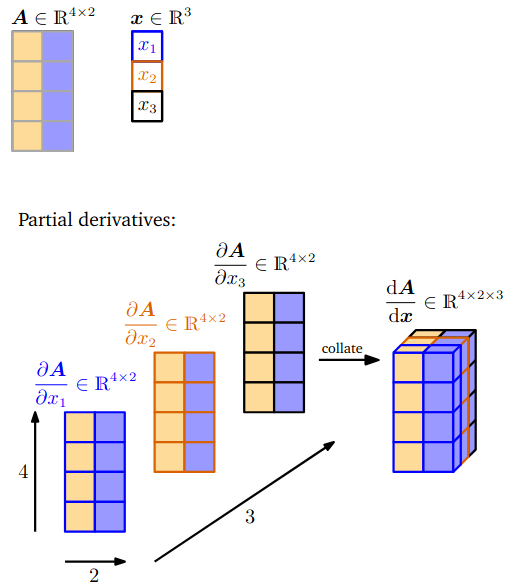
\includegraphics[
        width=\linewidth,
        height=5cm,
        keepaspectratio,
    ]{images/Vector-Calculus/Gradients-of-Matrices-approach1.png}
    \caption*{
        \textbf{Approach 1}: 
        We compute the partial derivative 
        $\dfrac{\partial \bm{A}}{\partial x_1}$ , 
        $\dfrac{\partial \bm{A}}{\partial x_2}$ , 
        $\dfrac{\partial \bm{A}}{\partial x_3}$ , each of which is a $4 \times 2$ matrix, 
        and collate them in a $4 \times 2 \times 3$ tensor.
        \cite{mfml/book/mml/Deisenroth-Faisal-Ong}
    }
\end{figure}
\end{minipage}
\hfill
\begin{minipage}{0.45\linewidth}
\begin{figure}[H]
    \centering
    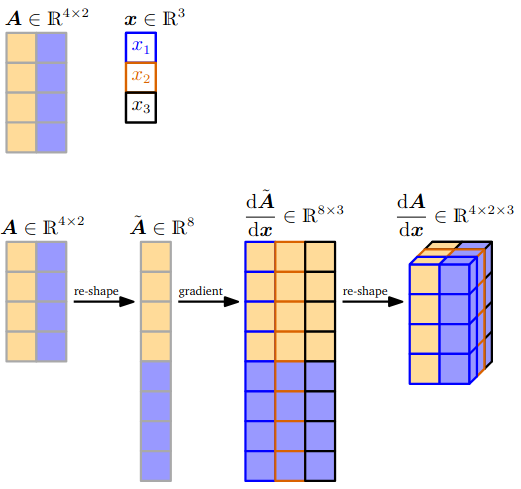
\includegraphics[
        width=\linewidth,
        height=5cm,
        keepaspectratio,
    ]{images/Vector-Calculus/Gradients-of-Matrices-approach2.png}
    \caption*{
        \textbf{Approach 2}: We re-shape (flatten) $\bm{A} \in \mathbb{R}^{4\times 2}$ into a vector $\tilde{\bm{A}} \in \mathbb{R}^8$. 
        Then, we compute the gradient $\dfrac{d\tilde{\bm{A}}}{d\bm{x}} \in \mathbb{R}^{8\times 3}$. 
        We obtain the gradient tensor by re-shaping this gradient as illustrated above.
        \cite{mfml/book/mml/Deisenroth-Faisal-Ong}
    }
\end{figure}
\end{minipage}
\hfill
\end{table}


\begin{enumerate}
    \item 
    \begin{definition}[Tensor]
        Tensor is a multidimensional array
        \hfill \cite{mfml/book/mml/Deisenroth-Faisal-Ong}
    \end{definition}

    \item 
    \begin{definition}[Flattening (matrix $\to$ vector)]
        Matrices can be transformed into vectors by stacking the columns of the matrix
        \hfill \cite{mfml/book/mml/Deisenroth-Faisal-Ong}
    \end{definition}

    \item if we compute the gradient of an $m \times  n$ matrix $\bm{A}$ with respect to a $p \times  q$ matrix $\bm{B}$, the resulting Jacobian would be $(m\times n)\times (p\times q)$, i.e., a four-dimensional tensor $\bm{J}$, whose entries are given as $J_{ijkl} = \dfrac{\partial A_{ij}}{\partial B_{kl}}$.
    \hfill \cite{mfml/book/mml/Deisenroth-Faisal-Ong}
\end{enumerate}










\section{Differentiation Rules}

\begin{enumerate}[series=vcalrules]
    \item \textbf{Product rule}: 
    \begin{enumerate}
        \item $
            (f(x)g(x))^\prime
            = \dfrac{d}{dx}(f(x)g(x))
            = g(x)\dfrac{d}{dx}f(x) + f(x)\dfrac{d}{dx}g(x)
            = f^\prime(x)g(x) + f(x)g^\prime(x)
        $
        \hfill \cite{mfml/book/mml/Deisenroth-Faisal-Ong}

        \item $
            \dfrac{\partial}{\partial \bm{x}}(f(\bm{x})g(\bm{x}))
            = g(\bm{x})\dfrac{\partial}{\partial \bm{x}}f(\bm{x}) 
                + f(\bm{x})\dfrac{\partial}{\partial \bm{x}}g(\bm{x})
        $ \hfill \cite{mfml/book/mml/Deisenroth-Faisal-Ong}
    \end{enumerate}

    \item \textbf{Quotient rule}:
    $
        \dParenBrac{\dfrac{f(x)}{g(x)}}^\prime
        = \dfrac{d}{dx}\dParenBrac{\dfrac{f(x)}{g(x)}}
        = \dfrac{f^\prime(x)g(x) - f(x)g^\prime(x)}{(g(x))^2}
    $
    \hfill \cite{mfml/book/mml/Deisenroth-Faisal-Ong}

    \item \textbf{Sum Rule}:
    \begin{enumerate}
        \item $
            (f(x) + g(x))^\prime
            = f^\prime(x) + g^\prime(x)
        $
        \hfill \cite{mfml/book/mml/Deisenroth-Faisal-Ong}

        \item $
            \dfrac{\partial}{\partial \bm{x}}(f(\bm{x}) + g(\bm{x}))
            = \dfrac{\partial}{\partial \bm{x}}f(\bm{x}) 
                + \dfrac{\partial}{\partial \bm{x}}g(\bm{x})
        $
        \hfill \cite{mfml/book/mml/Deisenroth-Faisal-Ong}
    \end{enumerate}

    \item \textbf{Chain Rule}: 
    \begin{enumerate}
        \item $
            (g(f(x)))^\prime
            = (g \circ f)^\prime(x)
            = g^\prime(f(x)) f^\prime(x)
        $
        \hfill \cite{mfml/book/mml/Deisenroth-Faisal-Ong}

        \item $
            \dfrac{\partial}{\partial \bm{x}}(g(f(\bm{x})))
            = \dfrac{\partial}{\partial \bm{x}}(g \circ f)(\bm{x})
            = \dfrac{\partial g(\bm{x})}{\partial f(\bm{x})}
                \dfrac{\partial f(\bm{x})}{\partial \bm{x}}
        $
        \hfill \cite{mfml/book/mml/Deisenroth-Faisal-Ong}
    \end{enumerate}
    $g \circ f$ denotes function composition $x \mapsto f (x) \mapsto g(f (x))$.
    \hfill \cite{mfml/book/mml/Deisenroth-Faisal-Ong}
\end{enumerate}

\vspace{0.5cm}
\textbf{Gradients of Matrices \& Vectors}:

\begin{multicols}{2}
\begin{enumerate}[resume*=vcalrules]
    \item $
        \dfrac{\partial \bm{f}(\bm{A})^\top}{\partial \bm{A}}
        = \dParenBrac{\dfrac{\partial \bm{f}(\bm{A})}{\partial \bm{A}}}^\top
    $
    \hfill \cite{mfml/book/mml/Deisenroth-Faisal-Ong}

    \item $
        \dfrac{\partial\ \tr(\bm{f}(\bm{A}))}{\partial \bm{A}}
        = \tr\dParenBrac{\dfrac{\partial \bm{f}(\bm{A})}{\partial \bm{A}}}
    $
    \hfill \cite{mfml/book/mml/Deisenroth-Faisal-Ong}

    \item 
    $
        \dfrac{\partial \bm{f}(\bm{A})^{-1}}{\partial \bm{A}}
        = -\bm{f}(\bm{A})^{-1}\ \dfrac{\partial \bm{f}(\bm{A})}{\partial \bm{A}} \ \bm{f}(\bm{A})^{-1}
    $ 
    \hfill \cite{mfml/book/mml/Deisenroth-Faisal-Ong}

    \item 
    $
        \dfrac{\partial\ \bm{x}^\top \bm{A}^{-1}\bm{y}}{\partial \bm{A}}
        = -(\bm{A}^{-1})^\top \bm{xy}^\top (\bm{A}^{-1})^\top
    $
    \hfill \cite{mfml/book/mml/Deisenroth-Faisal-Ong}

    \item 
    $
        \dfrac{\partial\ \bm{x}^\top \bm{A}\bm{y}}{\partial \bm{A}}
        = \bm{xy}^\top 
    $
    \hfill \cite{mfml/book/mml/Deisenroth-Faisal-Ong}

    \item 
    $
        \dfrac{\partial\ \bm{x}^\top \bm{A}\bm{x}}{\partial \bm{x}}
        = \bm{x}^\top(\bm{A} + \bm{A}^\top) 
    $
    \hfill \cite{mfml/book/mml/Deisenroth-Faisal-Ong}

    \item 
    $
        \dfrac{\partial\ \bm{x}^\top \bm{y}}{\partial\ \bm{x}} = \bm{y}^\top
    $
    \hfill \cite{mfml/book/mml/Deisenroth-Faisal-Ong}

    \item 
    $
        \dfrac{\partial\ \bm{y}^\top \bm{x}}{\partial\ \bm{x}} = \bm{y}^\top
    $
    \hfill \cite{mfml/book/mml/Deisenroth-Faisal-Ong}
\end{enumerate}
\end{multicols}

\vspace{0.5cm}
\begin{enumerate}[resume*=vcalrules]
    \item $
        \dfrac{\partial \det(\bm{f}(\bm{A}))}{\partial \bm{A}}
        = \det(\bm{f}(\bm{A}))\ \tr\dParenBrac{\bm{f}(\bm{A})^{-1}\ \dfrac{\partial \bm{f}(\bm{A})}{\partial \bm{A}}}
    $
    \hfill \cite{mfml/book/mml/Deisenroth-Faisal-Ong}

    \item 
    $
        \dfrac{\partial\ (\bm{x} - \bm{As})^\top \bm{W} (\bm{x} - \bm{As})}{\partial\bm{s}}
        = -2(\bm{x} - \bm{As})^\top \bm{WA}
    $
    \hfill
    (for symmetric $\bm{W}$)
    \hfill \cite{mfml/book/mml/Deisenroth-Faisal-Ong}
\end{enumerate}


\vspace{0.5cm}
\textbf{Examples}
\begin{enumerate}
    \item Consider a function $f : \mathbb{R}^2 \to \mathbb{R}$ of two variables $x_1, x_2$. 
    Furthermore, $x_1(t)$ and $x_2(t)$ are themselves functions of $t$. 
    \\
    $
        \nabla_t f(x_1, x_2)
        = \dfrac{df}{dt}
        = \begin{bmatrix}
            \dfrac{\partial f(x_1, x_2)}{\partial x_1(t)} &
            \dfrac{\partial f(x_1, x_2)}{\partial x_2(t)}
        \end{bmatrix}
        \begin{bmatrix}
            \dfrac{\partial x_1(t)}{\partial t} \\
            \dfrac{\partial x_2(t)}{\partial t}
        \end{bmatrix}
        = \dfrac{\partial f(x_1, x_2)}{\partial x_1(t)} \dfrac{\partial x_1(t)}{\partial t}
        + \dfrac{\partial f(x_1, x_2)}{\partial x_2(t)} \dfrac{\partial x_2(t)}{\partial t}
    $
    \hfill \cite{mfml/book/mml/Deisenroth-Faisal-Ong}

    \item If $f (x_1, x_2)$ is a function of $x_1$ and $x_2$, where $x_1(s, t)$ and $x_2(s, t)$ are themselves functions of two variables $s$ and $t$:
    \\
    $
        \begin{aligned}
        \nabla_{(s,t)} f(x_1, x_2)
        &= \dfrac{df(x_1, x_2)}{d(s,t)}
        = \dfrac{\partial f}{\partial \bm{x}} \dfrac{\partial \bm{x}}{\partial (s,t)}
        = \begin{bmatrix}
            \dfrac{\partial f(x_1, x_2)}{\textcolor{blue}{\partial x_1(s,t)}} &
            \dfrac{\partial f(x_1, x_2)}{\textcolor{green}{\partial x_2(s,t)}}
        \end{bmatrix}
        \begin{bmatrix}
            \textcolor{blue}{\dfrac{\partial x_1(s,t)}{\partial s}} & \textcolor{blue}{\dfrac{\partial x_1(s,t)}{\partial t}} \\
            \textcolor{green}{\dfrac{\partial x_2(s,t)}{\partial s}} & \textcolor{green}{\dfrac{\partial x_2(s,t)}{\partial t}}
        \end{bmatrix}
        \\
        &= 
        \begin{bmatrix}
            \dfrac{\partial f(x_1, x_2)}{\textcolor{blue}{\partial x_1(s,t)}}
            \textcolor{blue}{\dfrac{\partial x_1(s,t)}{\partial s}} +
            \dfrac{\partial f(x_1, x_2)}{\textcolor{green}{\partial x_2(s,t)}}
            \textcolor{green}{\dfrac{\partial x_2(s,t)}{\partial s}} \\ 
            \dfrac{\partial f(x_1, x_2)}{\textcolor{blue}{\partial x_1(s,t)}}
            \textcolor{blue}{\dfrac{\partial x_1(s,t)}{\partial t}} +
            \dfrac{\partial f(x_1, x_2)}{\textcolor{green}{\partial x_2(s,t)}}
            \textcolor{green}{\dfrac{\partial x_2(s,t)}{\partial t}}
        \end{bmatrix}
        \end{aligned}
    $
    \hfill \cite{mfml/book/mml/Deisenroth-Faisal-Ong}
    
\end{enumerate}




















\section{Backpropagation: Gradients in DNN}

\begin{table}[H]
\begin{minipage}{0.48\linewidth}
    \begin{figure}[H]
        \centering
        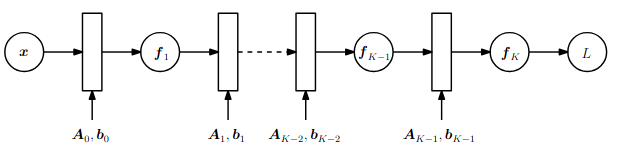
\includegraphics[
            width=\linewidth,
            height=3cm,
            keepaspectratio,
        ]{images/Vector-Calculus/sample-dnn-bp-ad.png}
        \caption*{
            Forward pass in a multi-layer neural network to compute the loss $L$ as a function of the inputs $\bm{x}$ and the parameters $\bm{A}_i, \bm{b}_i$.
            \cite{mfml/book/mml/Deisenroth-Faisal-Ong}
        }
    \end{figure}
\end{minipage}
\hfill
\vline
\hfill
\begin{minipage}{0.48\linewidth}
    \begin{figure}[H]
        \centering
        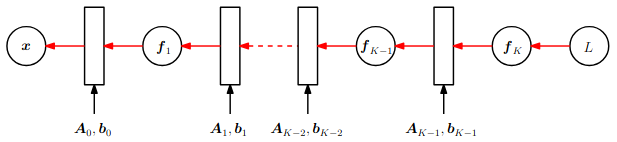
\includegraphics[
            width=\linewidth,
            height=3cm,
            keepaspectratio,
        ]{images/Vector-Calculus/sample-dnn-bp-ad2.png}
        \caption*{
            Backward pass in a multi-layer neural network to compute the gradients of the loss function.
            \cite{mfml/book/mml/Deisenroth-Faisal-Ong}
        }
    \end{figure}
\end{minipage}
\end{table}

\begin{enumerate}
    \item An area where the chain rule is used to an extreme is deep learning, where the function value $\bm{y}$ is computed as a many-level function composition 
    \hfill \cite{mfml/book/mml/Deisenroth-Faisal-Ong}
    \\
    .\hfill
    $
        \bm{y}
        = (f_K \circ f_{K-1} \circ \cdots \circ f_1)(\bm{x})
        = f_K (f_{K-1}(\cdots (f_1(\bm{x}))\cdots))
    $
    \hfill \cite{mfml/book/mml/Deisenroth-Faisal-Ong}
    \\
    where $\bm{x}$ are the inputs (e.g., images), $\bm{y}$ are the observations (e.g., class labels), and every function $f_i, i = 1, \cdots , K$, possesses its own parameters.
    \hfill \cite{mfml/book/mml/Deisenroth-Faisal-Ong}
    \\
    \begin{multicols}{2}
    \begin{enumerate}[series=grad-dnn]
        \item $\bm{f}_0 := \bm{x}$
        \hfill \cite{mfml/book/mml/Deisenroth-Faisal-Ong}

        \item $\bm{f}_i := \sigma_i(\bm{A}_{i-1}\bm{f}_{i-1} + \bm{b}_{i-1})$
        \hfill \cite{mfml/book/mml/Deisenroth-Faisal-Ong}

        \item $\bm{f}_i(\bm{x}_{i-1}) = \sigma_i(\bm{A}_{i-1}\bm{x}_{i-1} + \bm{b}_{i-1})$
        \hfill \cite{mfml/book/mml/Deisenroth-Faisal-Ong}

        \item $\bm{y} = \bm{f}_K(\bm{x}_{K-1})$
        \hfill \cite{mfml/book/mml/Deisenroth-Faisal-Ong}
    \end{enumerate}
    \end{multicols}
    \begin{multicols}{2}
    \begin{enumerate}[resume*=grad-dnn]
        \item $L(\bm{\theta}) = \dnorm{\bm{y} - \bm{f}_K(\bm{\theta},\ \bm{x})}^2$
        \hfill \cite{mfml/book/mml/Deisenroth-Faisal-Ong}
        
        \item 
        $
            \dfrac{\partial L}{\partial \bm{\theta}_{K-1}}
            = \dfrac{\partial L}{\partial \bm{f}_K} \textcolor{blue}{\dfrac{\partial \bm{f}_K}{\partial \bm{\theta}_{K-1}}}
        $
        \hfill \cite{mfml/book/mml/Deisenroth-Faisal-Ong}

        \item 
        $
            \dfrac{\partial L}{\partial \bm{\theta}_{K-2}}
            = \dfrac{\partial L}{\partial \bm{f}_K} 
            \textcolor{orange}{\dfrac{\partial \bm{f}_K}{\partial \bm{\theta}_{K-1}}}
            \textcolor{blue}{\dfrac{\partial \bm{f}_{K-1}}{\partial \bm{\theta}_{K-2}}}
        $
        \hfill \cite{mfml/book/mml/Deisenroth-Faisal-Ong}

        \item 
        $
            \dfrac{\partial L}{\partial \bm{\theta}_{K-2}}
            = \dfrac{\partial L}{\partial \bm{f}_K} 
            \textcolor{orange}{
                \dfrac{\partial \bm{f}_K}{\partial \bm{\theta}_{K-1}} 
                \cdots
                \dfrac{\partial \bm{f}_{i+2}}{\partial \bm{\theta}_{i+1}} 
            }
            \textcolor{blue}{\dfrac{\partial \bm{f}_{i+1}}{\partial \bm{\theta}_{i}}}
        $
        \hfill \cite{mfml/book/mml/Deisenroth-Faisal-Ong}
    \end{enumerate}
    \end{multicols}
    \begin{enumerate}
        \item [\textcolor{orange}{orange}] partial derivatives of the output of a layer with respect to its inputs

        \item [\textcolor{blue}{blue}] partial derivatives of the output of a layer with respect to its parameters
    \end{enumerate}
    \vspace{0.5cm}
    \textbf{where}:
    \begin{multicols}{2}
    \begin{enumerate}
        \item $i$: layer ($i = 1,\cdots,K$)
        \hfill \cite{mfml/book/mml/Deisenroth-Faisal-Ong}
        
        \item $\bm{x}_{i-1}$: output of layer $i - 1$
        \hfill \cite{mfml/book/mml/Deisenroth-Faisal-Ong}
        
        \item $\sigma_i$: activation function of layer $i$
        \hfill \cite{mfml/book/mml/Deisenroth-Faisal-Ong}

        \item $L$: loss function
        \hfill \cite{mfml/book/mml/Deisenroth-Faisal-Ong}

        \item $\bm{A}_{j},\ \bm{b}_{j}$: parameters ($j = 0,\cdots,K-1$)
        \hfill \cite{mfml/book/mml/Deisenroth-Faisal-Ong}

        \item $\bm{\theta} = \dCurlyBrac{\bm{A}_{0},\ \bm{b}_{0}, \cdots, \bm{A}_{K-1},\ \bm{b}_{K-1}}$
        \hfill \cite{mfml/book/mml/Deisenroth-Faisal-Ong}
    \end{enumerate}
    \end{multicols}

    \item 
\end{enumerate}





\section{Automatic Differentiation}

\begin{enumerate}
    \item Automatic differentiation is different from symbolic differentiation and numerical approximations of the gradient, e.g., by using finite differences.
    \hfill \cite{mfml/book/mml/Deisenroth-Faisal-Ong}
\end{enumerate}

























